\documentclass{mprop}
\usepackage{graphicx}

% alternative font if you prefer
%\usepackage{times}

% for alternative page numbering use the following package
% and see documentation for commands
%\usepackage{fancyheadings}


% other potentially useful packages
%\uspackage{amssymb,amsmath}
\usepackage{url}
%\usepackage{fancyvrb}
%\usepackage[final]{pdfpages}

\begin{document}

%%%%%%%%%%%%%%%%%%%%%%%%%%%%%%%%%%%%%%%%%%%%%%%%%%%%%%%%%%%%%%%%%%%
\title{Technical Debt Title Here}
\author{Ovidiu Popoviciu}
\date{18th December 2017}
\maketitle
%%%%%%%%%%%%%%%%%%%%%%%%%%%%%%%%%%%%%%%%%%%%%%%%%%%%%%%%%%%%%%%%%%%

%%%%%%%%%%%%%%%%%%%%%%%%%%%%%%%%%%%%%%%%%%%%%%%%%%%%%%%%%%%%%%%%%%%
\tableofcontents
\newpage
%%%%%%%%%%%%%%%%%%%%%%%%%%%%%%%%%%%%%%%%%%%%%%%%%%%%%%%%%%%%%%%%%%%

%%%%%%%%%%%%%%%%%%%%%%%%%%%%%%%%%%%%%%%%%%%%%%%%%%%%%%%%%%%%%%%%%%%
\section{Introduction}\label{intro}

\begin{itemize}
	\item What is technical debt?
	\item What are its applications?
	\item Why is it important?
\end{itemize}

Technical debt - is it real? How does it correlate with goals of the sprint?\\

Problem statement: Has the student analysed the problem, stated it clearly, and justified its importance?

%%%%%%%%%%%%%%%%%%%%%%%%%%%%%%%%%%%%%%%%%%%%%%%%%%%%%%%%%%%%%%%%%%%
\section{Statement of Problem}

Clearly state the problem to be addressed in your forthcoming project.\\

Explain why it would be worthwhile to solve this problem. \\

%%%%%%%%%%%%%%%%%%%%%%%%%%%%%%%%%%%%%%%%%%%%%%%%%%%%%%%%%%%%%%%%%%%
\section{Background Survey}
\subsection{Definition}

% Ward Cunningham - WyCash Portfolio Management System
Technical debt is a metaphor termed by Ward Cunningham, in his famous report on the WyCash Portfolio Management System in 1993 \cite{Cunningham1993}.
In the report, Cunningham mentioned that "\textit{shipping first time code is like going into debt.}" and that as the system evolves new features would become more and more difficult to implement.
This phenomenon was due to feature-rich projects being shipped to customers early but poorly written with little or no consideration to quality and to future work. 

% MTD 2010
The metaphor was ignored for a long time, until the late 2000s, when more and more studies started to look into the metaphor and explore its definition, identification process, measurement and management.
A figure of the popularity of Technical Debt from 2004 to present can be seen in Figure \ref{fig:td-trend}, information provided by Google Trends \cite{GoogleTrends}.
Thus, the first workshop on managing technical debt took place in 2010, where an initial research agenda was proposed for the future of software engineering field.
The workshop lasted 1 day and consisted of seminars, presentations and brainstorming sessions.
Technical debt workshops have been held every year since, and it in 2018 it will become a full 2-day conference.

\begin{figure}
	\centering
	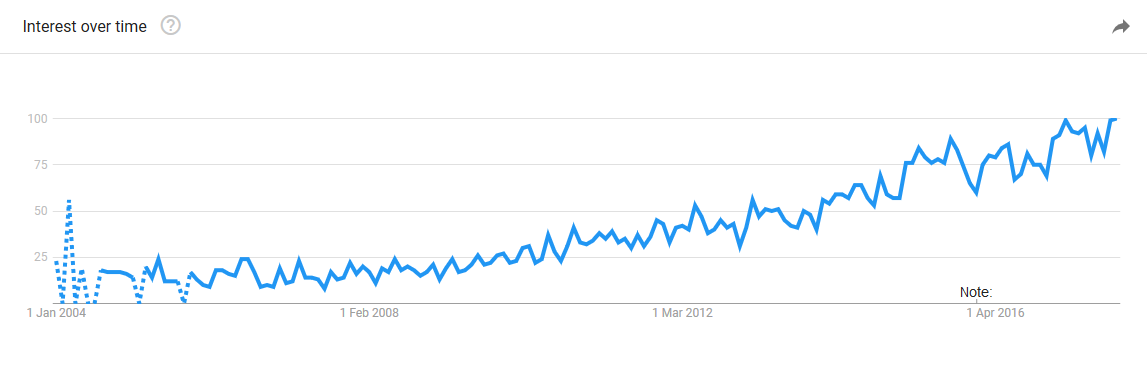
\includegraphics[width=\linewidth]{visualisations/TD_trend.png}
	\caption{Technical Debt Trend from 2004 to Present}
	\label{fig:td-trend}
\end{figure}


\subsubsection{MTD 2010 - Managing Technical Debt in Software Reliant Systems} \cite{Brown2010}
\begin{itemize}
	\item What were the goals of the paper? \\
	      The paper proposes a research agenda for the future of software engineering field.
	      It will allow developers, architects, managers and stakeholders to gain an edge in delivering high quality software without incurring any additional costs that come with the recurring interests of technical debt.
	      Using appropriate practices and tools, a complex aspect such as technical debt may be managed in a straightforward way.
	\item What was the methodology? \\
	      This was the first seminar of technical debt, in which numerous researchers brainstormed ideas for a few days and came up with an initial definition of technical debt, its properties and challenges.
	\item What were the conclusions? \\
	      The participants enumerated supposed properties of technical debt: value, visibility, present value, debt accretion, environment, origin of debt – intentional or unintentional, impact of debt.
	      Additionally, they have set up a few initial research questions for further study:
	      \begin{itemize}
		      \item How to assess the impact of TD quantitatively?
		      \item How to continously analize the structure of a project?
		      \item Which sources of debt are dominant, intentional or unintentional?
		      \item What is the cost of elimination? What are the visible consequences of holding on to that debt? What is the interest amount?
		      \item How can TD can be characterized in the context of decision making?
		      \item What are the appropriate toolings for quantifying and monitoring technical debt?
		      \item When is it appropriate to refactor and when to implement new features?
	      \end{itemize}
	\item Links to other resources?
\end{itemize}

\subsubsection{Technical Debt: From Metaphor to Theory and Practice} \cite{Kruchten2012}
\begin{itemize}
	\item What were the goals of the paper? \\
	      The goal of the article was to propose a view on how TD can be appplied within the software development practice and to identify the types of debt and ways to manage them.
	\item What was the methodology? \\
	      -
	\item What did the authors learn? \\
	      There were numerous learnings and conclusions drawn from the article.
	      First of all, there is a danger in associating technical debt with the metrics of static analysis tools that SD teams use daily, since those tools may not take into consideration large amounts of TD such as architectural debt.
	      Additionally, the authors have considered that TD is not only about code and code quality. For example, no tool will reveal poor choices made 2 years ago in terms of which technology to use. \\

	      Second of all, TD can also be incurred by technology gaps between development teams, product managers and stakeholders.
	      These gaps in technology is a result of context evolution over time, such as decision that might have been appropriate when they have been put in practice but which have slowly incurred debt over time.\\

	      Third of all, future decisions and changes have the most impact on software projects.
	      There are many questions unanswered in terms of how to manage technical debt from a future perspective:
	      \begin{itemize}
		      \item How to decide which changes to make in the next sprint and in which sequence?
		      \item How can these decisions be quantified from a financial point of view?
	      \end{itemize}
	      The finance issue relates mostly to the \textit{cost-value ratio}, and can be related to other financial models such as the Net Present Value (NPV) and Total Cost of Ownership.

	      Finally, the authors consider that technical debt is still considered a technical issue and should be mainly managed from the development team which must deal with it on a daily basis.
	      Therefore, it is best for developers to list TD items in the team's issue tracker such that they can be picked up during development activity and can be considered in the sprint planning meetings.
	\item Links to other resources? \\
	      Theodoropoulos et al. \cite{Theodoropoulos2011} has created a definition of technical debt in terms of gaps between development teams and business and proposed ways to bridge these invisible gaps.
\end{itemize}

\subsubsection{Technical Debt from a Stakeholder\'s Perspective} \cite{Theodoropoulos2011}

\begin{itemize}
	\item What were the goals of the paper? \\
	      To create a definition of technical debt that better aligned with stakeholder interests and to bridge the technical gap between technology team and stakeholdes when managing software quality.
	\item What was the methodology?
	      This was a position paper, no methodology has been defined.
	\item What did the authors learn?
	      \begin{itemize}
		      \item Stakeholders generally care little about software quality, unless it is directly impacting their costs at the present time.
		      \item Software quality characteristics are interdependent, deferring quality maintenance in one area may affect other areas of quality. For example, deferring work within UX may impact usability and require users to find workarounds. Additionally, inadequate validation of data at one layer may affect downstream processes.
		      \item They provided a definition of technical debt, as follows: \textit{Technical debt is any gap within the technology infrastructure or its implementation which has a material impact on the required level of quality.}
		      \item An interesting idea was that technical debt should only be associated with costs within technology environment rather than business and process environment. Thus the term \textbf{technical} debt.
	      \end{itemize}
	\item Links to other resources? \\
	      How is Quality Evaluated? David Garvin, ISO Quality Attributes
\end{itemize}

\subsubsection{On the limits of the technical debt metaphor} \cite{Schmid2013}
\begin{itemize}
	\item What were the goals of the paper? \\
	      The goal was to identify shortcomings in the technical debt metaphor and find points where the analogy to the finance world breaks down.
	\item What was the methodology? \\
	      The authors have compared the applications of the word \textit{debt}, with finance roots, within the technical world.
	\item What were the conclusions? \\
	      They discovered that the analogy breaks down when it comes to:
	      \begin{itemize}
		      \item Unit of measurement - in finance there is a clear measurement of principal and interest through the use of monetary currencies. TD currently lacks this.
		      \item Fixed time period - debt items have a fixed \textit{maturity} date, whereas TD is not fixed and does not go away.
		      \item Fixed interest - debt items have a fixed interest that is paid monthly. However, dynamic interest characterizes TD best, since its impact depends on future decisions and development.
	      \end{itemize}
	      The perspective of technical debt is heavily influenced by what is considered in future development.
	      This also implies that what is considered \"good structure\" or \"clean code\" also relates to future development since future decisions influence current impact.
	      Unfortunately there is no such thing as a debt-free system. The authors claimed that adressing all problems on purely structural grounds relates to \textbf{gold-platting} the system.
	      Additionally, combined evaluation procedure of code, architectural and for other types of debt requires care sine TD may be overly estimated.
	\item Links to other resources? \\
	      S. Freeman. “Bad code isn’t Technical Debt, it’s an unhedged Call Option”. Blogpost at http://www.higherorderlogic.com/2010/07/bad-code-isnt-technical-debt-its-an-unhedged-calloption/
\end{itemize}

%%%%%%%%%%%%%%%%%%%%%%%%%%%%%%%%%%%%%%%%%%%%%%%%%%%%%%%%%%%%%%%%%%%
\subsection{Identification}

\subsubsection{On the role of Requirements in Understanding and Managing Technical Debt} \cite{Ernst2012}
\begin{itemize}
	\item What were the goals of the paper? \\
	      The goal of the paper was to describe technical debt within project requirements, including gathering and change management phases.
	\item What was the methodology? \\
	      The authors created a tool, RE-KOMBINE, that structure requirements as goals, targets and desired properties of the system.
	      They are bucketed into high-level and low-level objectives, and each had an assigned set of tasks which led to a solution.
	      The system had the ability to manage evolving requirements by changing the assigned tasks of the goals.
	\item What did the authors learn?\\
	      The relationship between TD in requirements and TD in implementation can be described in terms of product value.
	      If the product does not bring value to customers, implementation TD does not matter.
	      If implementation TD is high, then delivering value is extremely difficult.\\
	      The authors have defined TD in requirements as follows:\\
	      \textit{Technical debt in requirements process is the distance between the original solution S for a requirement R, and the changed requirement R} \\
	      The conclusions of the paper was that requirements must be refined at the very start of the project/work week/sprint so that no extra development effort is put into satisfying it.
	      If the requirements are not gathered correctly then implementation may not bring value to the customers.
	      The proposed solution was to insist on requirements forecasting from an early stage at the expense of extra costs.
	\item What were the limitations of the study?\\
	      The system has not been evaluated in the industry environment.\\
	      Requirements TD is not TD per se, but a measure of how the system changes over time with regards to its requirements gathering process.
	\item Links to other resources? \\
\end{itemize}


%%%%%%%%%%%%%%%%%%%%%%%%%%%%%%%%%%%%%%%%%%%%%%%%%%%%%%%%%%%%%%%%%%%
\subsection{Measurement}

\subsubsection{The SQALE Method for Measuring Technical Debt} \cite{Letouzey2012}

\begin{itemize}
	\item What were the goals of the paper? \\
	      The goal of this paper was to propose a standardized, language-agnostic framework for assessing the quality of source code by deriving measures for important code characteristics and calculating technical debt.
	\item What was the methodology? \\
	      The framework proposed consisted of four concepts:
	      \begin{itemize}
		      \item Quality Model - defines internal properties of code through a structured three-layer hierarchy (characteristic, sub-characteristic and requirement).
		      \item Analysis Model - measurement of the distance between the current state of the application and the \"optimized\" state, the quality target.
		      \item Indices - each characteristic of the Quality Model defines a remediation index (cost to repair the non-compliances) defined in time, work or capital units.
		      \item Indicators - provide a visual representation of technical debt either through ratings (ratios between TD and development cost) or SQALE Pyramids (distribution of TD over all the characteristics).
	      \end{itemize}
	\item What did the authors learn?
	      \begin{itemize}
		      \item Each organization must manage technical debt as early as possible in a project with indicators and dashboards for code quality available for each build within the continous integration pipeline.
		      \item Quality model must be calibrated according to the requirements and policies of the organization implementing the framework. For example, to approve/decline rules that are considered debt and what principal costs are for each type of code violation.
		      \item One limitation is that the framework does not take into consideration other types of technical debt such as requirements debt, operational debt.
		      \item There is no standardized definition of right code, organizations have to define their own \"right\" code rules.
	      \end{itemize}
	\item Links to other resources?
	      -
\end{itemize}

\subsubsection{Estimating the Size, Cost and Types of Technical Debt} \cite{Curtis2012}
\begin{itemize}
	\item What were the goals of the paper? \\
	      Summarized the results of a study on a huge database (365M LOC) of software projects across 10 industries.
	      The study was language agnostic and provided a formula for estimating the principal of TD items.
	\item What was the methodology? \\
	      Made use of CAST's Application Intelligence platform to statically analyse source code, using 1200 rules for good practices.
	      The steps taken were as follows: parsing, identify violations, aggregate results and sum up into a quality characteristics, or \textit{health factors}.
	      Scores from each health factor were aggregated on a scale of 1 (high risk) to 4 (low risk).
	      The principal was estimated by a formula with three parameters: number of problems, time required for each fix and the cost of fixing the issue.
	\item What were the conclusions? \\
	      The authors concluded that estimating the interest incurred by a TD item was difficult since might be multiple hidden factors which influenced the results.
	      The term works well with the phenomenon since stakeholders think of software quality in terms of business. \\
	      There are trade-offs of TD management from stakeholder's perspective.
	      For example, fixing TD items within the Robustness characteristic may lead to fewer operational failures and higher availability of the system.
	\item What were the limitations? \\
	\item Links to other resources? \\
\end{itemize}

\subsubsection{An Empirical Model of Technical Debt and Interest}  \cite{Nugroho2011}

\begin{itemize}
	\item What were the goals of the paper? \\
	      The goal was to formally define technical debt and interest to provide insights on the Return On Investment (ROI) of IT executives.
	      Specifically, it tried to answer the following questions from a financial perspective: How large is TD? How much interest are paying? What are the consequences of holding on to debt?
	\item What was the methodology? \\
	      The authors had completed an empirical analysis of 44 projects within the Software Improvement Group (SIG) using TUViT software quality assessment method for collecting relevant metrics: lines of code, code duplications, etc.
	      The had also defined technical debt as being the changes needed to bring a system from its current quality state to the "ideal" quality. This can be quantified as the repair effort (RE) and can be calculated as follows:
	      RE = Rework Fraction (LOC need to be changed) * Rebuild Value (estimate in man-months of rebuilding with a particular technology) * Refactoring Adjustment (advanced tooling helping the team be more productive.)\\
	      The interest was also derived from the extra cost spent on maintainance per month and per year, modelled against the quality factor (the current state of quality within the system).
	\item What did the authors learn?
	      Maintainance was considered a different activity by the authors since the tasks involved in maintaining a system involve a change that is immediately visible from the outside.
	      However, technical debt repair was not considered a maintainance activity.
	      A few limitations of this approach were the level of precision rating of a system (quality ratings are on a scale of 1-5) which leads to less accurate estimations on important financial numbers such as ROI.
	      Refactoring adjustment variable is subjective as it requires expert input when considering development productivity.
	\item Links to other resources? \\
	      - S. McConnell. 10x software development \\
	      - Maintainability measurement - I. Heitlager, T. Kuipers, and J. Visser. A practical model for measuring maintainability. In Quality of Information and Communications Technology, 2007. QUATIC 2007. 6th International Conference on the, pages 30–39. IEEE, 2007.
	      - Eick, T. Graves, A. Karr, J. Marron, and A. Mockus. Does code decay? assessing the evidence from change management data. Software Engineering, IEEE Transactions on, 27(1):1–12, 2002.
\end{itemize}

\subsubsection{Investigating the Impact of Design Debt on Software Quality} \cite{Zazworka2011}
\begin{itemize}
	\item What were the goals of the paper? \\
	      To investigate the impact God classes have on development and whether they are points of major changes and defects when compared to other parts of the system. Additionally, to study whether there is a linear relationship between class size, change and defect likelihoods and how the results are influenced by data normalizations

	\item What was the methodology?
	      The authors ran an analysis on two medium-sized projects from a small development company. The analysis consisted of statically analysing the source code stored in version control and the project issues from the project management system.
	      It looked at two major variables:
	      \begin{itemize}
		      \item Change likelihood = how likely code within and outside God classes changes accross revisions.
		      \item Defect likelihood = how likely is a fix implemented inside and outside of God classes.
	      \end{itemize}
	\item What did the authors learn?
	      Empirical analysis of the two projects has shown that God classes get changed 7.8\% of the time whilst also being fixed 17 times more than the rest of the code.
	      However, since the God classes have more functionality included, normalization of the data by LOC has shown that there are no significant results in comparing God vs non-God classes.
	      The limited scope of the empirical analysis on a sample of two projects and focus on a specific code smell, the results are indecisive for a generalization of the results.
	\item Links to other resources?
\end{itemize}

\subsubsection{Investigating the impact of Code Smells Debt on Quality Code Evaluation} \cite{Fontana2012}
\begin{itemize}
	\item What were the goals of the paper? \\
	      The goals were to study the impact on code quality metrics of removing code smell, which code smell incurs the most TD and whether their impact on is related to the domain of the software application.
	      Should code smells be categorized as design debt?
	\item What was the methodology? \\
	      The study looked at three most common smells: Data class, God class and Duplicated Code.
	      The metrics impacted are related to cohesion, coupling and complexity; calculated by various tools according to clarity of computation.
	      Best refactoring practices were applied for each smell detected in the system and the quality metrics have been re-analysed to assess their impact.
	\item What did the authors learn? \\
	      Some code quality tools evaluate code smells through a set of rules which must be customized according to the application domain of the system.
	      Refactoring of one code smell may provide benefits for one or more metric qualities but may negatively impact others.
	      Additionally, code duplication is one of the worst smells but may also provide benefits in some cases.
	      Data Class smell and God class smells may be domain-dependent, but this assumption heavily correlates with the types of tools and libraries listed as dependencies in the system.
	\item Links to other resources? \\
	      Zhang et al. investigated relationship between code smells and software faults => how to prioritize refactoring.\\
	      Arcelli et al. proposed a first analysis on refactoring on a small scale of software metrics.
\end{itemize}

\subsubsection{Monitoring Code Quality and Development Activity by Software Maps} \cite{Bohnet2011}
\begin{itemize}
	\item What were the goals of the paper? \\
	      The goal of the paper was to bridge the gap between development teams and corporate managers, by exposing internal system quality through the use of software maps.
	      Software maps enable managers to assess where improvement in quality is most necessary and can observe future quality risk and estimate future maintenance costs.
	      Additionally, it helps developers and project managers identify modules suitable for refactoring/clean-up before the start of a sprint.
	\item What was the methodology? \\
	      A software map is a hierarchical 2D/3D view of software artefacts within a project.
	      Each artefact is represented visually through properties such as colour, texture and size; each representing a property of quality: cyclomatic complexity, LOC, nesting levels.
	      The authors have implemented a software for visualizing software maps and evaluated the tool on two projects: JBoss and Blender.
	\item What were the conclusions? \\
	      The authors have defined the internal quality of the system to be directly correlated to the quality of the source code.
	      These qualities are invisible to customers and management, and stakeholders are reluctant to put more resources into internal quality.
	      On the other hand, external quality relates to the visible, discoverable qualities of the system.
	      For example, defects and bugs are two discoverable phenomenons of external quality.
	      Impact of external quality issues are immediate, and stakeholders are inclined to invest in quick features/fixes that make an instant impact.
	\item What were the limitations? \\
	      The system has not been evaluated in practice.\\
	      There is no aggregation of values into a single metric that is understandable by both parties.\\
	      Calculating the cost of a change is difficult, only shows the past and current quality status.
	\item Links to other resources? \\
\end{itemize}

%%%%%%%%%%%%%%%%%%%%%%%%%%%%%%%%%%%%%%%%%%%%%%%%%%%%%%%%%%%%%%%%%%%
\subsection{Management}

\subsubsection{A Portfolio Approach to Managing Technical Debt} \cite{Guo2011}

\begin{itemize}
	\item What were the goals of the paper?\\
	      To define technical debt from a financial portfolio perspective by encouraging to be viewed as an investment and therefore used as a strategy.
	      Which TD items should be paid in a release for a particular component \textit{S}?
	\item What was the methodology?\\
	      The authors were looking at debt items in a system similar to assets in a financial portfolio, looking to maximize return on investment and minimize the risk associated with TD items.
	      In short, they were interested to find out whether an optimal combination of assets (TD items) can be found. \\
	      An approach proposed was to identify historical metrics of TD items and decide which ones to keep (the ones on which to pay interest) and which ones to sell (which to pay the principal i.e. FIX).
	\item What did the authors learn? \\
	      Technical debt is not problematic unless the costs outweight the benefits.
	      The approach does not take into consideration the fact that TD items may be recklessly added to the "portfolio" and the management of undetected TD items.
	      Additionally, technical debt is not the same as financial debt. The amount of principal and interest are known before hand and fixed in finance whereas in software development estimation is one of the most difficult tasks.
	      Approach was not tested in a real setting.
	\item Links to other resources?
\end{itemize}

\subsubsection{Prioritising Design Debt Investment Opportunities} \cite{Zazworka2011Prioritise}
\begin{itemize}
	\item What were the goals of the paper? \\
	      Proposes an approach for making refactoring decision regarding God classes in software projects, that will have a low principal cost and long-term benefits.
	\item What was the methodology? \\
	      The authors have considered the cost-benefit analysis criteria for prioritization, by taking into consideration the cost of refactoring and quality gained from each refactoring of TD items.
	      The proposed method approximates size of refactoring based on source code complexity metrics such as Weighted Method Count, Tight Class Cohesion and Access to Foreign Data Metric.
	      A feasibility study was conducted on a small size software development company on a project with 35k LOC, 11 month old and mantained by a team of 4 developers.
	\item What were the limitations of the study? \\
	      There were no results related to the feasibility study.
	      The study was only conducted on a single class smell, the God class.
	      Choice of refactoring must also be evaluated by the business side.
	\item Links to other resources? \\
\end{itemize}


\subsubsection{Using Technical Debt Data in Decision Making} \cite{Seaman2012}
\begin{itemize}
	\item What were the goals of the paper? \\
	      To discuss the approaches of technical debt management and to propose four novel ways to aid decision making.
	\item What were the conclusions? \\
	      Proposed four approaches for decision making on TD:
	      \begin{itemize}
		      \item Cost-Benefit Analysis. Defined principal, interest probability (the probability that other work will be more expensive) and the interest amount.
		            Based on these three factors and their associated value (high, medium, low), the authors claimed it is possible to estimate items that have low principal (are quick to repay) and a possible high impact on future additions and changes.
		      \item Analytic Hierarchy Process (AHP). Defined a criteria by which TD items would be paid off, through group decisions.
		      \item Portfolio Approach. Guo et al. \cite{Guo2011} has defined an approach for portfolio debt management. The same approach has been defined here.
		      \item Options. Represents investments into refactoring as a purchase of options that will facilitate change in the future but with no immediate profit.
	      \end{itemize}
\end{itemize}

%%%%%%%%%%%%%%%%%%%%%%%%%%%%%%%%%%%%%%%%%%%%%%%%%%%%%%%%%%%%%%%%%%%
\subsection{Industry Case Studies}

\subsubsection{What Software Practitioners have to say about TD} \cite{Lim2012}
\begin{itemize}
	\item What were the goals of the paper? \\
	      The goals of the study was to gather information on how practitioners identify, visualize and manage technical debt in industry.
	\item What was the methodology? \\
	      The authors have had interviews with 35 practitioners with broad backgrounds: various companies, a range of years of experiences, positions, etc.
	      The interview questions were both open-ended and closed-ended.
	\item What were the conclusions? \\
	      After being introduced to a definition of TD, 25\% of the participants considered TD as unintentional, and the rest considered that TD was caused by various trade-offs.
	      They understood that business reality forces trade-offs within software quality in order to satisfy business goals.
	      Furthermore, some practitioners mentioned that their team cut back on software quality enforcement methods due to time constraints and due to this TD was incurred in their projects.
	      They had to balance requirements and software quality against deadlines, since customer/business demands always took precedence. \\

	      However, participants have struggled to find a way to measure TD and its cumulative effort over time.
	      Moreover, convincing management to invest resources in paying back TD is difficult, unless there is an associated business value.
	      Unfortunately, there was no vocabulary defined between development teams and business, hence difficult to explain TD and its associated costs over time.
	      Some teams have had success in convincing stakeholders of the impact of TD, by quickly implementing a set of requirements and visualizing their trade-offs over a period of time.
	      As a result, they reported that stakeholders were happy to negotiate extending deadlines for features due to this. \\

	      The two perspectives of TD, from development to business, is different.
	      Developers are mainly interested in the perfection of the code whilst management considers that time to market is of extreme importance.
	      However, developers are more aware of the impact of TD over time, since they have to deal with it on a daily basis. \\

	      As a result of the study, the authors, developers and management have proposed the following practices when dealing with TD:
	      \begin{itemize}
		      \item Allocate 5-10\% of resources for each release in paying back TD.
		      \item Always keep an open dialogue with the customers and management on issues surrounding TD.
		      \item Make TD as visible as possible through the use of documentation, static analysis tools, etc.
	      \end{itemize}
	\item Links to other resources? \\
\end{itemize}

\subsubsection{Searching for Build Debt} \cite{Morgenthaler2012}
\begin{itemize}
	\item What were the goals of the paper? \\
	      To publish enterprise approaches within Google for managing technical debt in build files.
	      This type of TD was lowering developer productivity and increased the computational resources within the infrastructure and thus increased costs.
	\item What was the methodology? \\
	      The developers at Google leveraged in-door developed tools for automating removal of legacy code projects no longer refenced, removal of indirect dependencies between projects and removal of dead command-line flags which hindered developer comprehension of command line tools and processes.
	      Teams were holding FIXIT days where developers may remove and improve dead flags and dead/zombie dependencies.
	\item What were the conclusions? \\
	      Google has a very large codebase that is difficult to manage.
	      Specifically, a simple dependency change might take weeks due to previous links in the dependency graphs and build files of other projects that rely on it.
	      Removal of dead code has been simplied with the introduction of code visibility and health flags.
	      Additionally, one FIXIT day has removed approximately 250k lines of code related to dead flags.
	\item What were the limitations? \\
	      There was only one type of TD assessed in the paper: BUILD debt.
\end{itemize}

\subsubsection{Managing Technical Debt - An industrial case study} \cite{Codabux2013}
\begin{itemize}
	\item What were the goals of the paper? \\
	      The goals of the paper was to complete an empirical analysis of Agile methodologies and its effect on technical debt within a mid-sized company.
	      In particular, the authors wanted to find what were the various types of TD, how to handle them, what the consequences of holding on to that debt are, how TD is prioritized and addressed.
	\item What was the methodology? \\
	      The authors had 3 visits to the office of the company, each 3-day long.
	      They were part of team meetings such as sprint planning, scrum and retrospectives.
	      Interviews with both management and development teams have been completed.
	      A total of 28 members had participated to the study.
	\item What were the conclusions? \\
	      The authors had mixed responses when comparing division management interviews and developers.
	      Division management considered technical debt to be of infrastructure nature (in terms of operations) and testing nature (issues with test automation).
	      Developers, on the other hand, correlated TD with the lack of time to implement features \textit{properly}.\\
	      However, architecture debt was considered to be the most difficult to manage since it required group decisions which take time and coordination.
	      The team was taking appropriate steps to exterminate TD by assigning small teams within the division solely dedicated to refactoring tasks.
	\item What were the limitations? \\
	      The study was conducted with one industry partner and therefore does not reflect the impact of TD within the entire Agile process.
	      Additionally, interviews were not recorded and responses may be subject to bias of the interviewer.
	\item Links to other resources? \\
\end{itemize}

\subsubsection{Technical Debt and its Effects on Agile Management Practice} \cite{Holvitie2014}
\begin{itemize}
	\item What were the goals of the paper? \\
	      To study technical debt within the agile management process and its impact.
	\item What was the methodology? \\
	      The study consisted of three sections of research questions which covered background information and TD knowledge level, agile processes affecting TD and singular instances of TD.
	      Data collection was completed through an anonymous online form sent to 507 individuals spanning more than 150 companies.
	      The survey consisted of 34 questions open and closed-ended and took approximately 10 minutes to complete.
	\item What were the conclusions? \\
	      80\% of the individuals have heard of technical debt before and considered to have a good knowledge on it.
	      Of their entire day, TD was discussed most in work meetings while only 35\% of the responses have applied refactorings related to TD.\\
	      50\% of the participants considered practices such as simple design, TDD, following code standards, continous integration, collective ownership and pair programming to have a positive effect on TD.
	      Additionally, of all the meetings, retrospectives have been considered as most influential to TD by 50\% of the responses.
	      However, phases such as requirements gathering, design and implementation had been considered to incur the most TD.
	\item What were the limitations? \\
	      The study was conducted online anonymously - no way to understand how many sectors, how many companies and teams have been involved in the responses.\\
	      Limited to the country of the authors - Finland.
\end{itemize}

\subsubsection{An Enterprise Perspective on Technical Debt} \cite{Klinger2011}

\begin{itemize}
	\item What were the goals of the paper? \\
	      To challenge Ward Cunningham's definition of technical debt from an enterprise perspective and define it as a strategic tool for business circumstances.
	\item What was the methodology? \\
	      Interviewed four technical architects from IBM, from a "wide range" of projects within the firm. Each interview was approx. 1 hour in length.
	      The questions tapped into their own experiences with TD, more specifically: nature and context, stakeholders, benefits, documentation, whether the debt was repaid.
	\item What did the authors learn? \\
	      Enterprises may use debt as a tool for maximizing competitive advantage, which may or may not be paid in the future dependant on the direction in which the project will take.
	      Additionally, many stakeholders are involved in the accrual of debt in a software project (decisions are made collectively, not in a vacuum) but sometimes technical decisions would be made ad-hoc with no definite formal process.
	      However, the challenge is in the collective - it is difficult to understand the socio-technical background of a system. \\

	      Some stakeholders do not comprehend the extent of technical debt they are incurring in the system through their decisions due to:
	      \begin{itemize}
		      \item No vocabulary between technical architects and non-technical stakeholders.
		      \item Stakeholders having competing goals and "win" conditions which may be "suboptimal from a technical perspective".
	      \end{itemize}
	\item Links to other resources?
\end{itemize}

%%%%%%%%%%%%%%%%%%%%%%%%%%%%%%%%%%%%%%%%%%%%%%%%%%%%%%%%%%%%%%%%%%%
\section{Proposed Approach}

state how you propose to solve the software development problem. Show that your proposed approach is feasible, but identify any risks.

Goal-Question-Metric approach is a good framework for breaking down research work.

Goal-Question-Metric approach:
\begin{itemize}
	\item Goal: \textbf{Analyze} project feature implementations \textbf{with the purpose of} identifying extra work \textbf{from the viewpoint of} software engineers and project manager \textbf{in the context of} technical debt management.
	\item RQ1: What is the impact of TD on feature implementation?
	\item RQ1.1: What was the initial estimated work and the actual work for a project task?
	\item RQ1.2: What is the measurement of technical debt within the area of implementation?
	\item RQ2: How many resources should a team invest in each iteration on refactoring?
	\item RQ2.1: What is the overall amount of extra work the team puts into on each iteration? i.e. \textbf{How much interest does the team pay on each iteration?}
	\item RQ2.2: What is the measurement of TD on a project level?
\end{itemize}

Possible approach:
1) Identify appropriate data candidates for this study.
2) Retrieve historical work items along with project plan data.
3) Identify checkpoints in project codebase which are appropriate to the selected work items.
4) Proceed with static analysis of checkpoints and gathering of metrics.
5) Analysis of the results.
6) Discussion and further work.

Risks:
1) Data candidates may not contain enough relevant information in project management software for this study, such as priority and story points. 
2) Change sets estimation is difficult in the context of open source systems. What metric can quantify work appropriately?
3) Tools of calculating TD metrics must be suit for purpose. What static analysis tool may deliver appropriate metrics?
4) Granularity of checkpoints is important (e.g. pull-request level to release level).

%%%%%%%%%%%%%%%%%%%%%%%%%%%%%%%%%%%%%%%%%%%%%%%%%%%%%%%%%%%%%%%%%%%
\section{Work Plan}

show how you plan to organize your work, identifying intermediate deliverables and dates.\\
\textbf{TBD}

%%%%%%%%%%%%%%%%%%%%%%%%%%%%%%%%%%%%%%%%%%%%%%%%%%%%%%%%%%%%%%%%%%%
\section{Conclusion}

Does it clearly explain the problem? 
Does it contain a bibliography and proper citations?

Report: Is the report complete, well-organised, clear, and literate? 
Overall: What is your overall impression of the student’s work?

%%%%%%%%%%%%%%%%%%%%%%%%%%%%%%%%%%%%%%%%%%%%%%%%%%%%%%%%%%%%%%%%%%%
% it is fine to change the bibliography style if you want
\bibliographystyle{plain}
\bibliography{mprop}
\end{document}
